% KU Leuven latex presentation template
%
% © 2012 Michael Hofmann
%
% This work is licensed under the Creative Commons Attribution 3.0 Unported License.
% To view a copy of this license, visit
% http://creativecommons.org/licenses/by/3.0/ or send a letter to Creative
% Commons, 444 Castro Street, Suite 900, Mountain View, California, 94041, USA.

\documentclass[t,12pt,dutch
\ifx\beamermode\undefined\else,\beamermode\fi
]{beamer}
%\setbeameroption{show notes}
%\setbeameroption{show only notes}

\usepackage[utf8]{inputenc}
\usepackage[T1]{fontenc}
\usepackage{amsmath}
\usepackage[nohyperlinks]{acronym}
\usepackage{babel,lmodern,graphicx,mathptmx,xspace,wasysym,microtype,booktabs,tabularx,relsize,textcomp,longtable,lipsum,colortbl,eurosym,url,multicol,etoolbox,multimedia,pdfpages,fixltx2e,ifluatex,epstopdf}
\usepackage[olditem,oldenum]{paralist}
\usepackage[babel=true]{csquotes}
\usepackage[thinqspace,amssymb,textstyle]{SIunits}
\usepackage[textsize=tiny]{todonotes}
\usepackage[symbol]{footmisc}
\usepackage[notquote]{hanging}
\usepackage[normalem]{ulem}
\usepackage[mathscr]{euscript}
%\usepackage{lua-visual-debug}

\pdfstringdefDisableCommands{\renewcommand{\sout}{}}
\graphicspath{{figures/}}
% Fix sort order in case the same file exists with multiple extensions
\DeclareGraphicsExtensions{.pdf,.png,.jpeg,.jpg,.eps}
\frenchspacing

\input{templates/definitions.tex}



%% From pandoc default template
%% End pandoc

\mode<presentation>

%\hypersetup{pdfpagemode=FullScreen}

\setbeamercolor{structure}{fg=kulbright}
\setbeamercolor{title}{fg=white}
\setbeamercolor{footline}{parent=title}
\setbeamercolor{normal text}{fg=kuldefault}
\setbeamercolor{item}{parent=normal text}
\setbeamercolor{section in toc}{parent=normal text}
\setbeamercolor{footline extra}{fg=white}
\setbeamerfont{title}{size=\Large}
\setbeamerfont{tiny structure}{series=\bfseries}
\setbeamerfont{caption}{}

\setbeamersize{text margin left=0.8cm}
\setbeamersize{text margin right=0.8cm}
\setbeamersize{sidebar width left=0cm}

\setbeamertemplate{navigation symbols}{}
\setbeamertemplate{itemize item}{\footnotesize\raise1pt\hbox{\textbullet}}
\setbeamertemplate{itemize subitem}{--}
\setbeamertemplate{itemize subsubitem}{\tiny\raise1.5pt\hbox{\textbullet}}

\setlength\leftmargini{1em}
\setlength\leftmarginii{1em}
\setlength\leftmarginiii{1em}

\defbeamertemplate{background canvas}{title}
{%
    \pgfdeclarehorizontalshading{bgshading}{8.70cm}{color(0cm)=(kulleft); color(\the\paperwidth)=(kulright)}%
    \vbox to 8.70cm{%
        \pgfuseshading{bgshading}\hspace*{-1.6cm}%
    }%
    \hskip-\paperwidth%
    \hskip1.6cm%
    \vbox to \paperheight{%
        \vskip0.5cm\hskip0.5cm\includegraphics[width=2.83cm]{templates/kuleuven}%
        \vskip0.99cm\hskip0.76cm\includegraphics[width=2.84cm]{templates/key}%
        \vskip-0.57cm\hskip11.61cm\includegraphics[width=0.58cm]{templates/sedes}\hspace*{-1cm}%
        \vfill
    }%
}

\defbeamertemplate{background canvas}{grid}
{%
    \begin{tikzpicture}[remember picture,overlay,every node/.style={anchor=center}]
        \foreach \d in {0,...,20} {
            \draw[gray] (\d,0) -- (\d,-20);
            \draw[gray] (0,-\d) -- (20,-\d);
            \draw[lightgray] (\d+0.5,0) -- (\d+0.5,-20);
            \draw[lightgray] (0,-\d-0.5) -- (20,-\d-0.5);
            \node[anchor=north,red,font=\tiny] at (\d,0) {\d};
            \node[anchor=west,red,font=\tiny] at (0,-\d) {\d};
        }
    \end{tikzpicture}
}



% add a macro that saves its argument
\newcommand{\footlineextra}[1]{\gdef\insertfootlineextra{#1}}
\newbox\footlineextrabox


% add a beamer template that sets the saved argument in a box.
% The * means that the beamer font and color "footline extra" are automatically added.
\defbeamertemplate*{footline extra}{default}{
    %\begin{beamercolorbox}[ht=2.25ex,dp=1ex,leftskip=\Gm@lmargin]{footline extra}
    \begin{beamercolorbox}[ht=0.37cm,dp=0.25cm,wd=0.4\paperwidth,left,leftskip=2ex]{footline extra}
    \insertfootlineextra
    %\par\vspace{2.5pt}
    \end{beamercolorbox}
}

\defbeamertemplate{background canvas}{plain}{}

\defbeamertemplate{footline}{large}
{%
    \pgfdeclarehorizontalshading{bgshading}{0.62cm}{color(0cm)=(kulleft); color(\the\paperwidth)=(kulright)}%
    \vskip.3cm% make room for the logo
    \parbox[t][0.62cm]{\paperwidth}{\pgfuseshading{bgshading}}\par%
    \vskip-0.62cm%
    \begin{beamercolorbox}[ht=0.37cm,dp=0.25cm,center]{page number in head/foot}%
    \insertframenumber%
    \end{beamercolorbox}%
    \vskip-0.92cm%
    \parbox[t][0.92cm]{\paperwidth}{\hskip10.33cm\includegraphics[width=2.10cm]{templates/kuleuven}}\par%

    % set the box with the extra footline material but make it add no vertical space
    \setbox\footlineextrabox=\vbox{\usebeamertemplate*{footline extra}}
    \vskip -\ht\footlineextrabox
    \vskip -\dp\footlineextrabox
    \box\footlineextrabox%
}

% patch \begin{frame} to reset the footline extra material
\makeatletter
\let\beamer@original@frame=\frame
\def\frame{\gdef\insertfootlineextra{}\beamer@original@frame}
\footlineextra{}
\makeatother


\defbeamertemplate{footline}{nopagenumber}
{%
    \pgfdeclarehorizontalshading{bgshading}{0.62cm}{color(0cm)=(kulleft); color(\the\paperwidth)=(kulright)}%
    \vskip.3cm% make room for the logo
    \parbox[t][0.62cm]{\paperwidth}{\pgfuseshading{bgshading}}\par%
    \vskip-0.62cm%
    \begin{beamercolorbox}[ht=0.37cm,dp=0.25cm,center,ignorebg]{page number in head/foot}%
    %
    \end{beamercolorbox}%
    \vskip-0.92cm%
    \parbox[t][0.92cm]{\paperwidth}{\hskip10.33cm\includegraphics[width=2.10cm]{templates/kuleuven}}\par%
}

\defbeamertemplate{footline}{small}
{%
    \vskip.3cm% make room for the logo
    \begin{beamercolorbox}[ht=0.37cm,dp=0.25cm,center,ignorebg]{normal text}%
    \mdseries\insertframenumber%
    \end{beamercolorbox}%
}

\setbeamertemplate{footline}[large]

\setbeamertemplate{frametitle}
{%
    \nointerlineskip%
    \vskip.28cm%
    {\usebeamercolor[fg]{framesubtitle}\usebeamerfont{framesubtitle}\insertsupertitle\strut\par}%
    \vskip-.2cm%
    {\usebeamercolor[fg]{frametitle}\usebeamerfont{frametitle}\insertframetitle\strut\par}%
    \vskip-.3cm%
}

\setbeamertemplate{title page}
{
    \vbox{}%
    \vskip2.8cm%
    \vbox to 6.5cm{%
        \hskip2.8cm%
        \begin{minipage}{7.9cm}
            \begin{beamercolorbox}{title}
                \usebeamerfont{title}%
                \inserttitle\par%
                \ifx\insertsubtitle\undefined%
                \else%
                    \vskip0.25em%
                    {\usebeamerfont{subtitle}\usebeamercolor[fg]{subtitle}\insertsubtitle\par}%
                \fi%
            \end{beamercolorbox}%
            \vskip1em\par
            \begin{beamercolorbox}{author}
                \usebeamerfont{author}\usebeamercolor[fg]{subtitle}%
                \insertauthor
            \end{beamercolorbox}
            \begin{beamercolorbox}{institute}
                \usebeamerfont{institute}\usebeamercolor[fg]{subtitle}%
                \insertinstitute
                \end{beamercolorbox}
            \begin{beamercolorbox}{date}
                \usebeamerfont{date}\usebeamercolor[fg]{subtitle}%
                \insertdate
            \end{beamercolorbox}%
        \end{minipage}%
        \vfill
    }
}

\mode<all>

\newcommand{\inlinesound}[2]{\movie[inlinesound,encoding=Signed,samplingrate=44100]{#1}{#2}}

% disable for now as otherwise all commands that go between frames generated by
% the filter will result in duplicate toc lines
\renewcommand{\addcontentsline}[3]{}

\newcommand{\largefooter}{\setbeamertemplate{footline}[large]}
\newcommand{\emptyfooter}{\setbeamertemplate{footline}[nopagenumber]}
\newcommand{\smallfooter}{\setbeamertemplate{footline}[small]}
\newcommand{\nofooter}{\setbeamertemplate{footline}[nofooter]}

\newcommand{\sectiontoc}{\AtBeginSection[]{{
    \nosupertitle
    \emptyfooter
    \begin{frame}[noframenumbering]{Outline}
                \tableofcontents[currentsection]
            \end{frame}
    \largefooter
}}}

\newcommand{\subsectiontoc}{\AtBeginSubsection[]{{
    \nosupertitle
    \emptyfooter
    \begin{frame}[noframenumbering]{Outline}
                \tableofcontents[currentsection,currentsubsection]
           \end{frame}
    \largefooter
}}}

\newcommand{\notoc}{\AtBeginSection[]{}\AtBeginSubsection[]{}}

\newcommand{\nosupertitle}{\renewcommand{\insertsupertitle}{}}
\newcommand{\sectiontitle}{\renewcommand{\insertsupertitle}{\insertsectionhead}}
\newcommand{\subsectiontitle}{\renewcommand{\insertsupertitle}{\insertsectionhead\ifx\insertsubsectionhead\empty\else{} -- \insertsubsectionhead\fi}}

% animations do not work atm as figures are set on independent frames
\newcommand{\slidefig}[2]{\usebackgroundtemplate{\parbox[c][\paperheight][c]{\paperwidth}{\centering\includegraphics#1[height=\paperheight,width=\paperwidth,keepaspectratio]{#2}}}\begin{frame}[plain]\end{frame}\usedefaultcanvas}

\newcommand{\usedefaultcanvas}{\setbeamertemplate{background canvas}[\defaultcanvas]}
\newcommand{\gridcanvas}{\renewcommand{\defaultcanvas}{grid}\usedefaultcanvas}
\newcommand{\plaincanvas}{\renewcommand{\defaultcanvas}{plain}\usedefaultcanvas}

\newcommand{\insertsupertitle}{}






\newcommand{\defaultcanvas}{plain}


% Defining a new coordinate system for the page:
%
% ----------------
% |(0,1)    (1,1)|
% |              |
% |(0,0)    (1,0)|
% ----------------
\makeatletter
\def\parsecomma#1,#2\endparsecomma{\def\page@x{#1}\def\page@y{#2}}
\tikzdeclarecoordinatesystem{page}{
    \parsecomma#1\endparsecomma
    \pgfpointanchor{current page}{north east}
    % Save the upper right corner
    \pgf@xc=\pgf@x%
    \pgf@yc=\pgf@y%
    % save the lower left corner
    \pgfpointanchor{current page}{south west}
    \pgf@xb=\pgf@x%
    \pgf@yb=\pgf@y%
    % Transform to the correct placement
    \pgfmathparse{(\pgf@xc-\pgf@xb)*\page@x+(\pgf@xb)}
    \expandafter\pgf@x\expandafter=\pgfmathresult pt
    \pgfmathparse{(\pgf@yc-\pgf@yb)*\page@y+(\pgf@yb)}
    \expandafter\pgf@y\expandafter=\pgfmathresult pt
}
\makeatother

% Example:
%\begin{tikzpicture}[remember picture,overlay,every node/.style={anchor=center}]
%  \node at (page cs:0.5,0.3) {0.5,0.3};
%  \node at (page cs:0,0) {0,0};
%  \draw(page cs:0,0) -- (page cs:1,1);
%  \draw[thick,red] (page cs:0,0) rectangle (page cs:1,1);
%  \draw[thick,green] (page cs:0.2,0.2) rectangle (page cs:0.8,0.8);
%\end{tikzpicture}

\setcounter{secnumdepth}{0}

\title{Hyperspectrale afbeeldingscompressie met tensordecomposities}
\author{\mbox{Wouter Baert} \and \mbox{Begeleider: Nick Vannieuwenhoven}}
\date{14 december 2018}
\institute{}


\begin{document}

\setbeamertemplate{background canvas}[title]

\begin{frame}[plain,noframenumbering]
    \titlepage
\end{frame}

\usedefaultcanvas


%\emptyfooter
%\begin{frame}[noframenumbering]{Outline}
%        \tableofcontents
%    \end{frame}
%\largefooter

%\section{First Section}\label{first-section}

% Slide 1-1
\begin{frame}{Hyperspectrale afbeeldingen}

\begin{figure}[H]
\centering
\includegraphics[scale=0.3]{images/cuprite_bands_1-44.png}
\caption{Cuprite, Nevada (VS): banden 1-44 (bron: AVIRIS)}
\end{figure}

\end{frame}

% Slide 1-2
\begin{frame}{Hyperspectrale afbeeldingen}

\begin{figure}[H]
\centering
\includegraphics[scale=0.3]{images/cuprite_bands_45-89.png}
\caption{Cuprite, Nevada (VS): banden 45-89 (bron: AVIRIS)}
\end{figure}

\end{frame}

% Slide 1-3
\begin{frame}{Hyperspectrale afbeeldingen}

\begin{figure}[H]
\centering
\includegraphics[scale=0.3]{images/cuprite_bands_90-134.png}
\caption{Cuprite, Nevada (VS): banden 90-134 (bron: AVIRIS)}
\end{figure}

\end{frame}

% Slide 1-4
\begin{frame}{Hyperspectrale afbeeldingen}

\begin{figure}[H]
\centering
\includegraphics[scale=0.3]{images/cuprite_bands_135-179.png}
\caption{Cuprite, Nevada (VS): banden 135-179 (bron: AVIRIS)}
\end{figure}

\end{frame}

% Slide 1-5
\begin{frame}{Hyperspectrale afbeeldingen}

\begin{figure}[H]
\centering
\includegraphics[scale=0.3]{images/cuprite_bands_180-224.png}
\caption{Cuprite, Nevada (VS): banden 180-224 (bron: AVIRIS)}
\end{figure}

\end{frame}

% Titelslide 1
\begin{frame}{}
\begin{center}
\topskip0pt
\vspace*{\fill}
\vspace*{\fill}
\Huge
Achtergrond
\normalsize
\vspace*{\fill}
\end{center}
\end{frame}

% Slide 2
\begin{frame}{Singulierewaardenontbinding (SVD)}

$A = U \Sigma V^T$ met 
\begin{itemize}
\item $A \in \mathbb{R}^{m \times n}$, $U \in \mathbb{R}^{m \times m}$, $\Sigma \in \mathbb{R}^{m \times n}$ en $V \in \mathbb{R}^{n \times n}$
\item $U$ en $V$ orthogonaal
\item $\Sigma$ diagonaal en positief, van groot naar klein
\newline
\end{itemize}
$A \approx \widetilde{U} \widetilde{\Sigma} \widetilde{V}^T$ met 
\begin{itemize}
\item $A \in \mathbb{R}^{m \times n}$, $\widetilde{U} \in \mathbb{R}^{m \times k}$, $\widetilde{\Sigma} \in \mathbb{R}^{k \times k}$ en $\widetilde{V} \in \mathbb{R}^{n \times k}$
\item $\widetilde{U}$, $\widetilde{V}$ eerste $k$ kolommen $U, V$
\item $\widetilde{\Sigma}$ eerste $k$ diagonaalelementen $\Sigma$
\item Beste rang-$k$ benadering van $A$ (Frobeniusnorm)
\end{itemize}

\end{frame}

% Slide 3
\begin{frame}{Tensoren en $n$-mode product (Kolda, Bader 2009)}

\begin{itemize}
\item $\mathscr{X}$ tensor met $d$ modes
\item $\mathscr{X} \times_k U$ met $U \in \mathbb{R}^{r_k \times n_k}$ betekent:
\begin{enumerate}
\item Neem vectoren volgens mode $k$ (lengte $n_k$)
\item Transformeer elke vector $x$ naar $Ux$ (lengte $r_k$)
\item Vouw terug in tensor
\end{enumerate}
\end{itemize}

\end{frame}

% Slide 4
\begin{frame}{Tucker-decompositie (Tucker 1963)}

\begin{itemize}
\item Stel $\mathscr{X}$ voor als tupel $(\mathscr{G} ; A_1, \dots, A_d)$ zodat $\mathscr{X} \approx \mathscr{G} \times_1 A_1 \dots \times_d A_d$ 
\\met $\mathscr{X} \in \mathbb{R}^{n_1 \times n_2 \times \dots \times n_d}$, $\mathscr{G} \in \mathbb{R}^{r_1 \times r_2 \times \dots \times r_d}$, $A_i \in \mathbb{R}^{n_i \times r_i}$
\item Compressieratio $\approx \frac{r_1 r_2 \dots r_d + n_1 r_1 + n_2 r_2 + \dots + n_d r_d}{n_1 n_2 \dots n_d}$
\item Voor hoge $d$: $\sim \prod_{i=1}^{d}\frac{r_i}{n_i}$
\end{itemize}

\end{frame}

% Slide 5
\begin{frame}{T-HOSVD (Tucker 1963)}

\begin{figure}[H]
\centering
\includegraphics[scale=0.3]{images/T-HOSVD.png}
\caption{Standaard T-HOSVD-algoritme (bron: Kolda, Bader 2009)}
\end{figure}

Niet zozeer beste Tucker-decompositie!

\end{frame}

% Slide 6
\begin{frame}{ST-HOSVD (Vannieuwenhoven, Vandebril, Meerbergen 2012)}

\begin{figure}[H]
\centering
\includegraphics[scale=0.25]{images/ST-HOSVD.png}
\caption{ST-HOSVD-algoritme (bron: VVM 2012)}
\end{figure}

\begin{itemize}
\item Sneller (sequentieel), zeker met goede modevolgorde
\item Bijna altijd betere benadering in de praktijk
\item Doelfout kan goed benaderd worden
\end{itemize}

\end{frame}

% Titelslide 2
\begin{frame}{}
\begin{center}
\topskip0pt
\vspace*{\fill}
\vspace*{\fill}
\Huge
Eigen onderzoek
\normalsize
\vspace*{\fill}
\end{center}
\end{frame}

% Slide 7
\begin{frame}{Optimalisatie ST-HOSVD}

\begin{itemize}
\item Beperkte sampling
\begin{itemize}
\item vb.: 314368 vectoren in dimensie 224 naar dimensie 12
\item Kan ook SVD van steekproef nemen
\item vb.: 24,8s $\rightarrow$ 6,7s voor volledige ST-HOSVD (fout quasi gelijk)
\item Singuliere waarden kunnen geschat worden
\end{itemize}
\item Gram-matrix
\begin{itemize}
\item SVD van $A \in \mathbb{R}^{m \times n}$ is eigenwaardenontbinding van $AA^T \in \mathbb{R}^{m \times m}$
\item $m \ll n$ dus veel sneller
\item Maar te grote numerieke fouten in de praktijk
\end{itemize}
\end{itemize}

\end{frame}

% Slide 8
\begin{frame}{Orthogonaliteitscompressie}

\begin{center}
$
\begin{bmatrix}
A & b & \dots \\[0.3em]
C & x & \dots \\[0.3em]
\end{bmatrix}
$
met $A \in \mathbb{R}^{(m-k) \times k}, C \in \mathbb{R}^{k \times k}, b \in \mathbb{R}^{m - k}, x \in \mathbb{R}^{k}$
\end{center}

\begin{itemize}
\item Orthogonaliteit $\Rightarrow C^T x = -A^T b$
\item Volledige driehoek herberekenen: numeriek problematisch
\end{itemize}

\noindent\begin{minipage}{0.7\textwidth}% adapt widths of minipages to your needs
Oplossingen:
\begin{itemize}
\item Blokken
\item Orthonormalisatie volledige kolom
\item Marge
\end{itemize}
\end{minipage}%
\hfill%
\begin{minipage}{0.3\textwidth}
\includegraphics[scale=0.8]{images/orthogonaliteitscompressie.png}
\end{minipage}

\end{frame}

% Slide 9
\begin{frame}{Quantisatie kerntensor}

\begin{figure}[H]
\centering
\includegraphics[scale=0.5]{images/values_per_layer.png}
\caption{log$_{10}$ van waarden per laag kerntensor}
\end{figure}

\end{frame}

% Slide 10
\begin{frame}{Quantisatie kerntensor}

\begin{itemize}
\item Grotere waarden op lagere indices
\item Impact fout op waarden overal gelijk
\end{itemize}
$\rightarrow$ Vast aantal bits per waarde, aparte quantizatiestap per laag kerntensor

\end{frame}

% Slide 11
\begin{frame}{Quantisatie factormatrices}

\begin{itemize}
\item Orthogonaal, dus elke waarde $\leqslant$ 1 en $\geqslant$ -1
\end{itemize}
$\rightarrow$ Vast aantal bits per waarde, vaste precisie voor alle waarden in alle factormatrices

\end{frame}

% Slide 12
\begin{frame}{Bitstring-compressie}

\begin{itemize}
\item Lossless compressie van uiteindelijke bitstring zonder interpretatie
\item DEFLATE-algoritme (gebruikt in zip, PNG, ...) via zlib-library
\end{itemize}

\end{frame}

% Slide 13
\begin{frame}{Globaal schema}
\vfill
\includegraphics[scale=0.19]{images/globaal_schema.png}
\end{frame}

% Titelslide 3
\begin{frame}{}
\begin{center}
\topskip0pt
\vspace*{\fill}
\vspace*{\fill}
\Huge
Resultaten
\normalsize
\vspace*{\fill}
\end{center}
\end{frame}

% Slide 14
\begin{frame}{Cuprite, Nevada (VS) (bron: AVIRIS)}

\begin{center}
\includegraphics[scale=0.5]{images/cuprite_0-025.png}
\end{center}

Relatieve fout: 2,69\%\\
Compressieratio: 2,51\%

\end{frame}

% Slide 15
\begin{frame}{Indian pines, Indiana (VS) (bron: AVIRIS)}

\begin{center}
\includegraphics[scale=0.5]{images/indian_pines_0-025.png}
\end{center}

Relatieve fout: 2,60\%\\
Compressieratio: 2,00\%

\end{frame}

% Slide 16
\begin{frame}{Okavango-delta, Botswana (bron: NASA)}

\begin{center}
\includegraphics[scale=0.5]{images/botswana_0-025.png}
\end{center}

Relatieve fout: 2,84\%\\
Compressieratio: 1,12\%

\end{frame}

% Slide X
\begin{frame}{Verder onderzoek}

\begin{itemize}
\item Variabele quantisatie factormatrices
\item Tensor trains
\item Blokgewijse compressie
\item Parameter tuning
\item DCT
\end{itemize}

\end{frame}

\end{document}
